\chapter{Basic Introduction}
\label{chapter1}
This tutorial will guide you through the basic features of StochSS. You will become familiar with the \textbf{Model Editor} and the \textbf{Simulation Manager}. You will learn how to create your own model, which can be population or concentration-based, and how to simulate it using either an ordinary differential equation (ODE) solver or the stochastic simulation algorithm (SSA).

\section{Creating Administrator and Standard User Accounts}
At the end of a successful installation process, your default browser will launch and you will be asked to create an admin account as in Figure \ref{fig:admin} (there is only one admin account for the entire system).
Once the admin account is created you will be forwarded to a regular login page where you can log in to StochSS.

\begin{figure}[!htb]
\centering
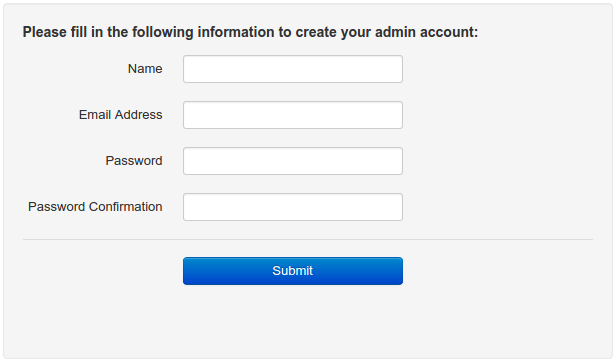
\includegraphics[scale=0.64]{T1/admin.png}
\caption{Administrator login page}
\label{fig:admin}
\end{figure}

Users can click \textbf{Create Account} to request an account.
The account will not be accessible until the admin approves it in the \textbf{Admin Panel} (the admin can also delete active users as well as reset their passwords there).
%
%\begin{figure}[!htb]
%\centering
%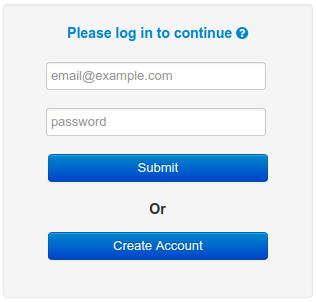
\includegraphics[scale=0.64]{T1/login.png}
%\caption{User login page}
%\label{fig:login}
%\end{figure}

\section{Importing a Model}
The \textbf{Model Editor} will let you create new or modify existing well-mixed stochastic biochemical models as well as deterministic models based on ODEs.
The best way to get started with the model editor is to import an example model and look at the different sections.

\subsection{Importing an existing model}

\underline{Option 1: StochSS Public Library}
\begin{itemize}
  \item Navigate to the \textbf{Model Editor} page.
  \item Click \textbf{Import from Public Library} in the right-hand toolbar.
  \item Select a model from the Public Library and click \textbf{Copy Model to Library}.
\end{itemize}

\noindent\underline{Option 2: Stochkit2 XML}
\begin{itemize}
  \item Navigate to the \textbf{Model Editor} page.
  \item Click \textbf{Import from .XML} in the right-hand toolbar.
  \item Select an XML file. A collection of example models can be found in the \textit{examples} directory within the StochSS install folder.
  \item Click \textbf{Import}.
\end{itemize}

After importing the XML file or public model, StochSS should display the imported model in the model editor.
Look through the page to see how the different \textbf{Species}, \textbf{Parameters}, and \textbf{Reactions} are defined.
By clicking \textbf{Export to .zip} or \textbf{Export to Public Library} the model can be shared across computers or shared amongst users of the same StochSS.

\section{Creating a New Model}
An example population model is defined by the following two reactions:
\begin{equation}
\label{eq:tut1-reac1}
\begin{aligned}
S0 + S0 &\xrightarrow{k1} S1\\
S1 &\xrightarrow{k0} \emptyset .  
\end{aligned}
\end{equation}

To create this model:
\begin{itemize}
  \item Navigate to the \textbf{Model Editor}.
  \item Click \textbf{Add Model} and select \textit{Population, Well-mixed}.
  \item Rename the model to \textit{example}.
  \item Click \textbf{Create Species} twice to create two species.
  \item By default the species are named $S0$ and $S1$. Set the initial condition for $S0$ to $1000$ and the initial condition for $S1$ to $0$.
  \item Similarly to above, click \textbf{Add Parameter} twice to add two parameters.
  \item By default they will be named $k0$ and $k1$. Set $k0$ to $0.0001$ and $k1$ to $0.05$.
  \item Click \textbf{Add Reaction} to add two reactions. Select the reactants, products, rates and reaction types corresponding to \eqref{eq:tut1-reac1}. Compare to Figures \ref{fig:reaction2} and \ref{fig:reaction1} to verify the settings.
\end{itemize}

\begin{figure}[!htb]
\centering
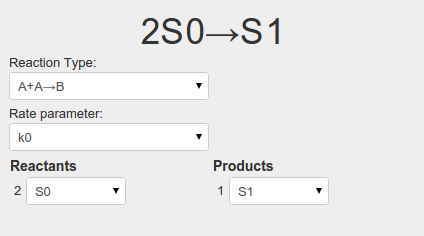
\includegraphics[scale=0.64]{T1/reaction2.png}
\caption{Dimerization reaction}
\label{fig:reaction2}
\end{figure}

\begin{figure}[!htb]
\centering
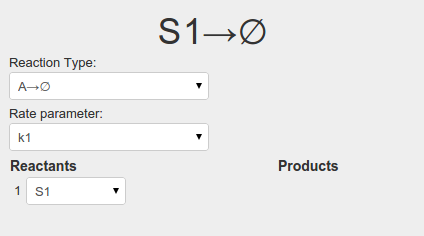
\includegraphics[scale=0.64]{T1/reaction1.png}
\caption{Decay reaction}
\label{fig:reaction1}
\end{figure}

\section{Running a Simulation and Visualizing results}

For this section, create or import a model using the directions above.

\begin{itemize}
  \item Navigate to the \textbf{Simulation Manager} page.
  \item Select the model you wish to simulate and click \textbf{Next}.
  \item Setup your simulation parameters: name, time, data storage frequency, realizations and solver type. 
  \begin{itemize}
    \item If you are simulating a population-based model you can choose between the deterministic and the stochastic solvers.
    %\item If you choose the deterministic solver, you have the possibility to perform sensitivity analysis on a set of chosen parameters related to your model.
    \item Concentration-based models can only be simulated using the deterministic solver.
  \end{itemize}  
  \item Click \textbf{Run Locally}. You will be automatically forwarded to the \textbf{Job Status} page.%When the job runs, StochSS should automatically transition to the \textbf{Job Status} page.
  \item Click \textbf{View} to open the \textbf{Job summary} page, where you can visualize the simulation's trajectories.
  \item Click \textbf{Access Local Data} to download a raw copy of the data. This can be used to share data between StochSS installations or perform manual data analysis.
\end{itemize}

\subsection{Converting a concentration model to population}
Create a concentration model or use the directions above to import one. Both Lotka-Volterra examples are concentration based and are available both as XML files and Public Library models.

\begin{itemize}
  \item Select the newly minted concentration model.
  \item Click \textbf{Convert to Population} on the right-hand toolbar to start the conversion process. The model conversion page will open.
  \item To convert a concentration model to a population, a system volume must be specified.
  \item Given a volume, StochSS converts initial conditions through 
  \begin{align}
  \mathrm{initial\_condition\_population} = \mathrm{initial\_condition\_concentration}\times\mathrm{volume}
  \end{align}
   and attempts to convert the reaction rates. It is not always possible to convert reaction rates automatically. If automatic conversion fails the conversion still proceeds, but the user now has to correct the reactions that were not automatically converted.
  \item Click \textbf{Finish conversion} at the bottom left of the page to create a population-based model. This newly created population model can be simulated using both deterministic and stochastic solvers.
  \item Click \textbf{Cancel conversion} to cancel the conversion.
\end{itemize}

\warning{The conversion process operates correctly only if the model to be converted is entirely based on the mass action kinetics allowed in Gillespie Stochastic Simulation Algorithm \cite{dan}. If the model to be converted is not entirely based on mass action kinetics, the conversion tool only converts what it can. }

\section{Backup and Transfer your Data}
You can backup or share your saved models and simulations with the StochSS ZIP format. There are three ways to create StochSS ZIP files:

\begin{enumerate}
\item Navigate to the \textbf{Backup} page in the left-hand toolbar and click \textbf{Export}. This exports a ZIP containing all models and simulation results for the current user. There is an option to export all data for all users if this page is accessed with the admin account.
\item Select a model on the \textbf{Model Editor} page and click \textbf{Export to .zip}.
\item Click \textbf{View} on the \textbf{Job Status} page, and then click \textbf{Access local data}.
\end{enumerate}

These ZIP files can all be imported into StochSS on the \textbf{Backup} page. To import the contents of a ZIP file into StochSS:

\begin{itemize}
\item Navigate to the \textbf{Backup} page.
\item Click \textbf{Import}.
\item Select the ZIP file to upload. The file should automatically begin uploading, and then appear in a table of ZIP archives below.
\item Select the ZIP file in the table.
\item Define the behavior of the import by either limiting what files get imported or specifying how overlapping names are handled.
\item Click \textbf{Import} at the bottom of the page.
\end{itemize}

\subsection{Exporting data from an old version of StochSS (1.2 or previous)}
To create a backup archive from an older version of StochSS, execute the following command from a terminal window in the directory of your new StochSS installation:
\begin{verbatim}
./exportserver.py path_to_your_old_StochSS_installation
\end{verbatim}
You can import the backup archive you created as described above.

